%%# -*- coding:utf-8 -*-

\documentclass[fontset=windows]{article}
% if you need to pass options to natbib, use, e.g.:
%     \PassOptionsToPackage{numbers, compress}{natbib}
% before loading neurips_2022


% ready for submission
% \usepackage{neurips_2022}


% to compile a preprint version, e.g., for submission to arXiv, add add the
% [preprint] option:
%     \usepackage[preprint]{neurips_2022}

\PassOptionsToPackage{numbers, compress}{natbib}  % ref https://arxiv.org/abs/2209.09407
% to compile a camera-ready version, add the [final] option, e.g.:
\usepackage[final]{neurips_2022}

% to avoid loading the natbib package, add option nonatbib:
%    \usepackage[nonatbib]{neurips_2022}

\usepackage[UTF8]{ctex}
\usepackage[T1]{fontenc}    % use 8-bit T1 fonts
\usepackage{hyperref}       % hyperlinks
\usepackage{url}            % simple URL typesetting
\usepackage{booktabs}       % professional-quality tables
\usepackage{amsfonts}       % blackboard math symbols
\usepackage{nicefrac}       % compact symbols for 1/2, etc.
\usepackage{microtype}      % microtypography
\usepackage{xcolor}         % colors
\usepackage{graphicx}       %%  图片包
\usepackage{subfig}
\usepackage{geometry}
\usepackage{calligra}
\usepackage{algorithm}
\usepackage{algorithmicx}
\usepackage{algpseudocode} 
\usepackage{amsmath}
\usepackage{amssymb}
\usepackage{bm}
\usepackage{multirow}
\usepackage{diagbox}
\usepackage{hyperref}
\usepackage{tablefootnote}
\usepackage{indentfirst}
\setlength{\parindent}{2em}
\newtheorem{definition}{Definition}[section]
\newtheorem{theorem}{Theorem}[section]
\newtheorem{notations}{Notations}

\title{音视频编码技术期末报告 -- 多类图像去雾复现}


% The \author macro works with any number of authors. There are two commands
% used to separate the names and addresses of multiple authors: \And and \AND.
%
% Using \And between authors leaves it to LaTeX to determine where to break the
% lines. Using \AND forces a line break at that point. So, if LaTeX puts 3 of 4
% authors names on the first line, and the last on the second line, try using
% \AND instead of \And before the third author name.


\author{%
    刘昭炀\\ %\thanks{Use footnote for providing further information
    电子与信息工程学院\quad 信息与通信工程专业\\
    22215608\\
    \href{mailto:liuzhy86@mail2.sysu.edu.cn}{liuzhy86@mail2.sysu.edu.cn}\\
}


\begin{document}
{

\maketitle

\begin{abstract}
    \indent 由于大气颗粒对光的散射,在恶劣天气(例如阴霾、雾、薄雾、烟雾)下拍摄的图像的颜色,对比度发生变化、能见度降低,图像信息发生了不可逆的变化。这些退化不仅会影响图像的视觉质量;更重要的是它们会改变图像中所包含的重要信息内容,进而降低一些室外视觉系统以及一些计算机视觉算法的性能。所以恶劣天气条件下的图像增强、图像复原有着切实的应用价值。单图像去雾(single image dehazing,SID)方法用于从单个模糊图像恢复可见性。由于其病态性质,SID 是一个具有挑战性的问题。通常,大气散射模型(atmospheric scattering model,ATSM)用于解决SID问题。传输和介质透射率(大气光)是ATSM的两个主要参数,基于大气散射物理模型的SID算法聚焦于如何更好地估计这两个参数,以获取更好的图像复原效果。

    \indent 本文主要复现了几种基于大气散射物理模型的传统方法去雾算法,它们各自拥有不同的优势(速度、成像效果),流程大同小异。在本文最后,对比了不同算法的效果。本文复现的源码可见于Github。\footnote{源代码可见于:\url{https://github.com/AnnLIU15/img_process/tree/SID}}
\end{abstract}

% footnote ref: https://arxiv.org/pdf/2108.10026.pdf
\begingroup
\let\clearpage\relax
\section{引言}
在户外的视觉智能系统中,常常会遇到可见性的问题,光照引起的问题会导致视觉智能系统性能极具下降,比如在夜晚中使用基于白天光照条件设计、训练出来的视觉系统,其表现会急剧下降甚至无法正常使用。除了夜晚这类光照强度问题外,不同的天气也会不同程度导致场景画面的能见度降低,从而影响了户外智能系统的性能。

本文复现的算法针对的就是有雾场景下的图像处理,大气粒子散射和吸收从物体表面反射的光。这种散射和吸收在恶劣天气下变得严重,导致辐照度的大小不正确,图像与视频会因为雾的存在导致性能急剧下降,图像出现退化的情况。相机接收到一小部分直接从物体表面反射的光,以及大量被大气粒子反射的光。因此,物体的对比度和可见性会减弱。户外视觉智能系统在我们的生活生产中遍地可见,如物体检测和识别、视觉监控、交通监控、智能交通。但是,由于图像和视频的退化,视觉智能系统表现不佳。因此,视觉智能系统需要一种方法解决雾对图像的影响。早期的去雾方法基于附加信息。这些方法需要如深度线索、偏振度等额外信息,需要通过用户交互或各种相机定位操作提供。因此,这些方法不适用于实时视觉应用。基于多幅图像的方法也需要从不同偏振度、不同天气场景下拍摄的多幅图像。这些方法需要额外的硬件或其他资源。因此,这些方法比SID计算代价更高,SID算法具有很强的实用性,胜任实时性要求高的场景。%\section*{References}

\section{去雾算法理论方法}
\label{s2}

\subsection{雾与霾的成因及影响}
雾,是一种常见的气象,被称为在地面上的云。当潮湿的空气中遇到灰尘等凝结核时,水蒸气会凝结,在冷凝过程中,水蒸气分子结合形成悬浮在空气中的小水滴与小冰晶,雾需要一定的湿度才会形成。雾可能会突然形成,然后很快消失。霾,是指原因不明的因大量烟、尘等微粒悬浮而形成的浑浊现象。霾的核心物质是空气中悬浮的灰尘颗粒,气象学上称为气溶胶颗粒,与雾不同的是,霾在干燥的时候更容易出现。

当烟、尘等微粒累积超过大气的调节能力时,雾霾就会在微风与大气稳定的情况下出现。由于存在大气吸收和散射,霾、雾和烟雾的现象,入射光与大气光混合,环境光被大气粒子反射到视线中。图像出现退化的问题,失去对比度和色彩保真度。雾与霾不但影响人的身心健康,还会影响基于视觉系统的各类服务,影响生活生产的各方各面,在生产、安全等方面存在巨大隐患。因此,图像去雾算法拥有巨大的需求。

\subsection{大气散射物理模型}
\label{subsec-atsm}
\begin{figure}[htbp]
    \centering
    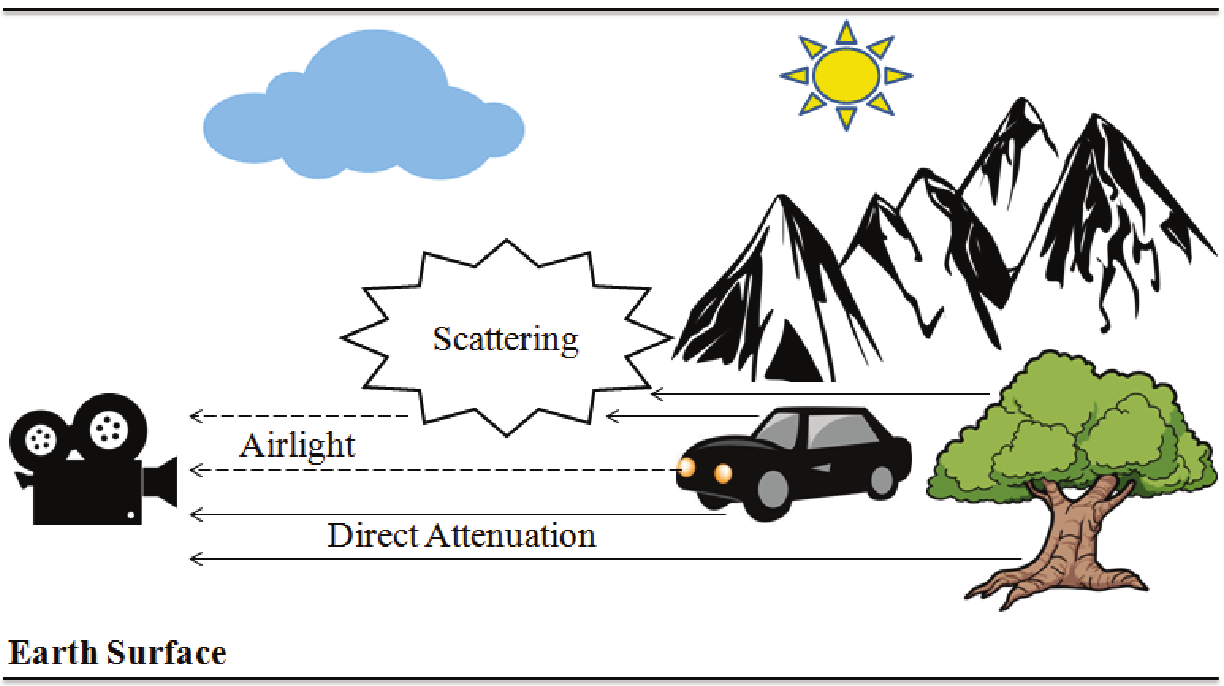
\includegraphics[width=0.8\textwidth]{./imgs/g167.png}
    \caption{大气散射物理模型}
    \label{fig-astm}
 \end{figure}

解决SID的基本模型是ATSM\cite{narasimhan2004models}。 ATSM考虑了散射光对恶劣天气下图像形成的影响。恶劣天气下的成像过程如图\ref{fig-astm}所示。物体表面反射入射的太阳光。一部分反射光到达相机(直接衰减),一部分反射光被大气粒子散射(大气光)。因此,相机接收到的图像是散射光和非散射光的总和。 ATSM模型可转化为数学表示\cite{narasimhan2004models},如公式\eqref{eq-astm}所示。

\begin{equation}
    I_h^c(x,y) = \underbrace{I_n^c(x,y)\times t_r(x,y)}_{\text{传输衰减}} + \underbrace{A_r^c(x,y)\times t_r(x,y)}_{\text{大气光}}
    \label{eq-astm}
\end{equation}

其中,$(x,y)$是图像中像素点的坐标,$c\in\text{(red,green,blue)}$是颜色通道,$I_n$是无雾图像,$I_h$是雾化图像,$A_r$是全局值大气光。位置 $(x,y)$处的透射率(非散射光比例)由 $t_r (x, y)$ 表示。公式\eqref{eq-astm2}描述了光如何在大雾天气中传输。

\begin{equation}
    t_r (x, y) = e^{-\gamma\text{Depth}(x, y)}
    \label{eq-astm2}
\end{equation}

其中,$0\leq\text{Depth}(x, y)\leq\infty$为场景点的景深,$\gamma$是散射系数。公式\eqref{eq-astm2}中可知随着景深的增大传输到相机的光减小。 SID 的主要任务是从单个模糊图像\cite{he.tang201112}估计 $t_r (x, y)$ 和$A_r$。将$t_r (x, y)$和$A_r$的值代入公式\eqref{eq-astm}即可得到无雾图像。无雾图像由于传输$t_r (x, y)$和附加大气光 $A^c_r\times (1 − t_r (x, y))$产生退化。因此,高质量SID非常需要准确的估计传输函数。雾度的浓度的估计由公式\eqref{eq-astm2}中的 $\gamma$ 和 Depth$(x,y)$控制。现有的去雾方法使用公式\eqref{eq-astm}或\eqref{eq-astm2} 来估计 $t_r (x, y)$。然而,由于估计的$A_r$和DCP在某些区域(如天空)的无效性,公式\eqref{eq-astm}引入了重建误差,同时公式\eqref{eq-astm2}的$\gamma$也会造成传输误差,也是一个重要的超参数,$\gamma$设置的合理与否直接影响传输函数的估计效果(默认为1)。

\subsection{去雾效果评价方法}
与其他计算机视觉的领域不一样,图像去雾效果的评价较为特殊,各个算法中的度量指标并不统一,没有一个严格的评价标准,但是大体上都分为两部分:主观评价和客观评价。

\subsubsection{主观评价方法}
主观评价的方法是依赖于观察测试人员的直观感受评价,评价一张图像处理后的质量,需要对多个观察测试人员的评价进行归一化即为该图像的评分。在图像去雾中,主观评价方法可分为两种,一种是对合成有雾图像的去雾评价,像这样有参照的无雾图像的属于绝对评价方法;另一种是对真实情况的有雾图像的去雾评价,像这样没有参照的无雾图像的属于相对评价方法。观察者根据自身对图像的视觉感受、图像质量、颜色与细节的模糊程度来判断去雾效果。虽然主观评价方法原理简单又能直接体现去雾效果,但是碍于观察测试者的自身情况不同,评价的标准也不尽相同,并且操作起来费时费力,导致主观评价并不能精准的反映去雾效果,也很难应用在类似于无人驾驶的实时图像去雾上。

\subsubsection{客观评价方法}
本文的客观评价方法主要基于两个计算机视觉中常用的度量:峰值信噪比(Peak Signal to Noise Ratio,PSNR)与结构相似性(Structural Similarity Index,SSIM)\cite{Zhou2004}。客观评价避免了人为主观的影响,并且对每一副图像都有相同的评价,可以批量处理与综合评价,反映整体去雾水平。在客观评价的实验中,我们采用了RESIDE\cite{li2019benchmarking}\footnote{https://sites.google.com/view/reside-dehaze-datasets/reside-standard}中的SOTS(Synthetic Objective Testing Set)户外数据集,数据集包括原图与加雾图,对去雾算法的评价方式为:结果客观评价方法的大致步骤就是,将处理后的图像作为输入,经客观评价模型计算后,再与无雾图像在数据上进行分析评价,如图\ref{fig6}所示。

\begin{figure}[htbp]
   \centering
   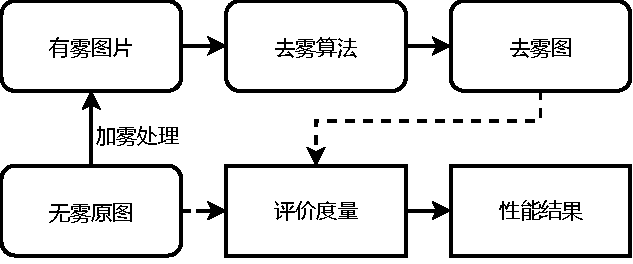
\includegraphics[width=0.8\textwidth]{./imgs/metric.pdf}
   \caption{客观评价方法流程图}
   \label{fig6}
\end{figure}


PSNR是客观评价方法的一种鉴别图像处理结果的画质的客观方法,可以看作评价图像的客观标准。表达式如公式\eqref{eq-psnr}所示:

\begin{equation}
    \text{MSE} = \frac{1}{MN\times\text{channels}}\sum\limits_{\dim}^{\text{channels}}\sum\limits_{i}^{M}\sum\limits_{j}^{N}(I_x^{(i,j,\dim)} -I_y^{(i,j,\dim)})^2,
    \label{eq-mse}
\end{equation}

\begin{equation}
    \text{PSNR} = 10\times\log_{10}\left(\frac{(2^n-1)^2}{\text{MSE}}\right).
    \label{eq-psnr}
\end{equation}

由上式可知,PSNR在作为图像品质的指标的时候,其实是均方误差(mean square error,MSE)\eqref{eq-mse}的一种变体,其中MSE的$n$指的是图像的位数。去雾后的图像与原图越相近,均方误差越小,PSNR 的值越高。图像去雾任务中,输出的图像和原图像会存在很大不同,PSNR 的大小无法和人评
价图像质量的视觉感受完全一致,有时候人眼看去雾效果差的图像,其 PSNR 分
数反而会相对较高。但是在这是因为人对图像某一区域的视觉感知结果会收到区域周围
的对比度、亮度等影响

SSIM是衡量两幅图像相似程度的指标,它的数值代表了两个图像之间的相似性。人类对像素的绝对亮度/颜色不敏感,但对边缘和纹理的位置非常敏感。SSIM通过主要关注边缘和纹理相似性来模仿人类感知。其表达式如公式\eqref{eq-ssim}所示:
\begin{equation}
    \hbox{SSIM}(I_x,I_y) = \frac{(2\mu_x\mu_y + c_1)(2\sigma_{xy} + c_2)}{(\mu_x^2 + \mu_y^2 + c_1)(\sigma_x^2 + \sigma_y^2 + c_2)}.
    \label{eq-ssim}
\end{equation}
其中$\mu_x$和$\mu_x$是图像像素集合$I_x$与$I_y$的平均像素亮度,$\sigma_x^2$与$\sigma_y^2$是$I_x$与$I_y$的方差,$\sigma_{xy}$是$I_x$与$I_y$的协方差;$c_1 = (k_1L)^2$, $c_2 = (k_2L)^2$是两个常数,确保除法中不存在除以0的情况,$L$是像素的取值范围(亮度格式)、默认情况下$ k_1 $$k_2 $的值分别为$0.01$与$0.03$.

在客观评价去雾效果时候,需要结合PSNR和SSIM两个评价指标,共同衡量去雾效果的优劣。
\section{单图像去雾}
\label{s3}



基于大气模型的SID算法的流程基本上大同小异,我复现以下的几种算法也是一样,一般来说这类SID的流程如图\ref{fig-dehazy}所示,其中边界函数的计算只在一些算法中采用。

\begin{figure}[htbp]
    \centering
    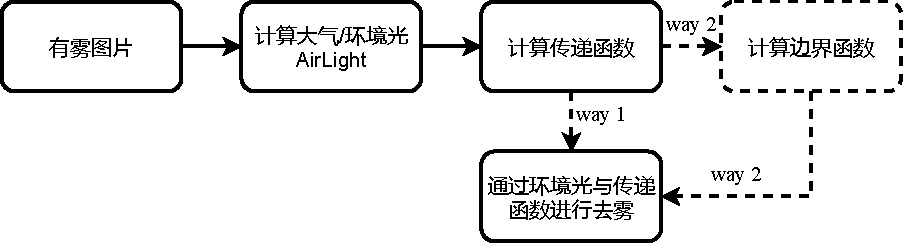
\includegraphics[width=0.8\textwidth]{./imgs/dehazy.pdf}
    \caption{去雾算法流程}
    \label{fig-dehazy}
 \end{figure}

\subsection{基于暗通道先验知识的单图像去雾}
何恺明团队在2009年的CVPR会议中提出暗通道先验(dark channel prior,DCP)算法(后发到TPAMI\cite{he.tang201112})。他们经过大量实验发现,除了亮区或天空区DCP是完全黑暗的,在所有的颜色通道中至少存在一个接近0的亮度值的像素。导致这种现象的原因为:每一张图片中不同物体互相遮挡形成的阴影、图像包括一个颜色接近RGB纯色的区域或者图片的整体风格接近于黑色。



首先我们对暗通道做一个定义,对于任意图像$I^c(x,y)$,其暗通道图像为$I_d^c(x,y)$,$I_d^c(x,y)$计算的过程如公式\ref{eq-dark}所示:
\begin{equation}
    I_d^c(x,y) = \text{minimum filter}(\min\limits_{c\in{r,g,b}}I_h^c(x,y)),
    \label{eq-dark}
\end{equation}
其中, minimum filter操作可由最小滤波器($3\times3$腐蚀)完成,即对每个通道最小值进一步最小滤波处理。他们大量实验发现,如果$I^c(x,y)$是室外无雾图像,除天空区域外,$I^c(x,y)$的暗通道$I_d^c(x,y)$每个像素的亮度较低且趋于零,即$I_d^c(x,y)\rightarrow0$,他们将此观察称为先验暗通道。

\begin{figure}[htbp]
    \centering
    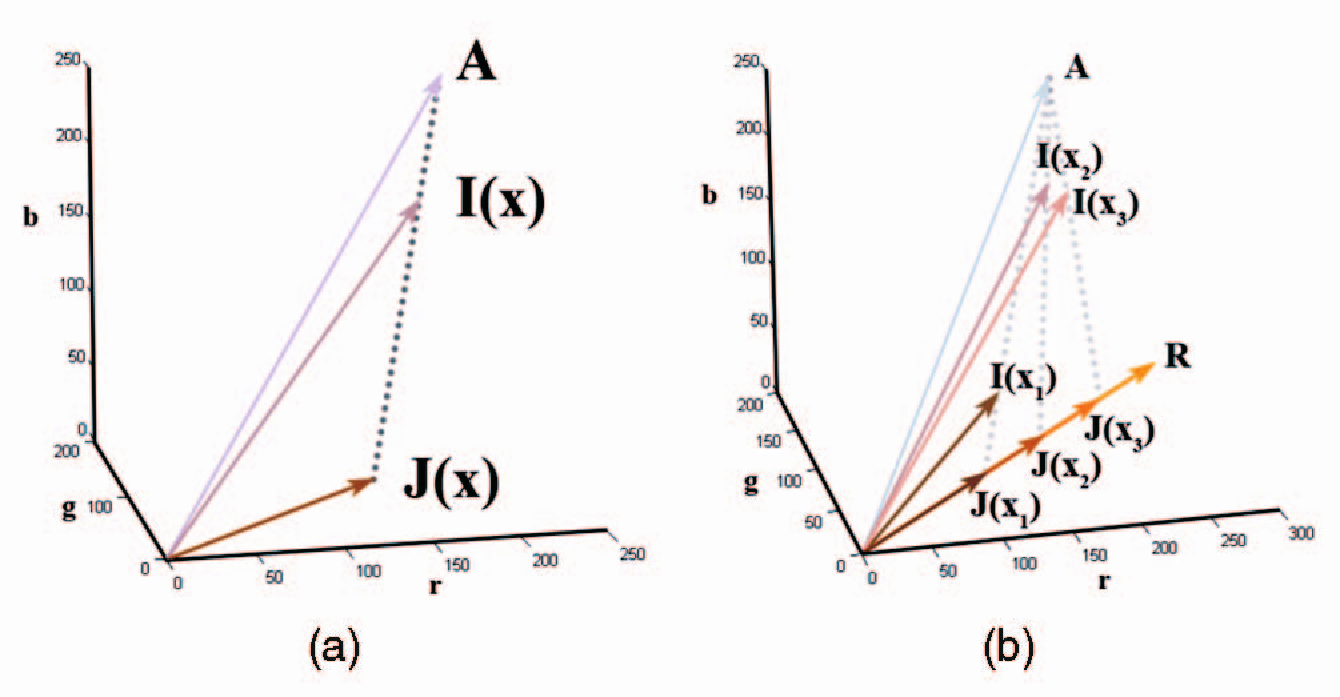
\includegraphics[width=0.8\textwidth]{./imgs/g711.png}
    \caption{传递函数}
    \label{fig-trans-dark}
 \end{figure}

去雾的传递函数与大气光以及暗通道的关系如公式\eqref{eq-trans-dark}所示,其在线性空间的表示可见于图\ref{fig-trans-dark}。

\begin{equation}
    t_r(x,y) = \frac{A_r^c - I^c(x,y)}{A_r^c - I_d^c(x,y)}
    \label{eq-trans-dark}
\end{equation}

根据图\ref{fig-dehazy}的流程,我们可以编写出该算法伪代码\ref{algo-DCP}。

\begin{algorithm}[t]
    \caption{DCP}
    \label{algo-DCP}
    \textbf{输入:} 有雾图像$I_h^c(x,y)$,滤波器核大小$W$,透视雾保留系数$\omega$,导向滤波器半径$r$,估计大气光使用的像素比例$p$
    \begin{algorithmic}
    \State 使用灰度化有雾图像$I_g^c(x,y)$计算有雾图像暗通道$I_d^c(x,y)$,根据暗通道 $I_d^c(x,y)$,获取最小$pMN\dim$个像素的位置
    \State 根据有雾图像中对应的位置的像素值估计每个通道的$A_r^c$
    \State 估计传递函数$\hat t_r(x,y) = 1 - \omega \min\limits_{c\in{r,g,b}}\frac    {I_h^c(x,y)}{A_r^c}$
    \State 对传递函数进行导向滤波$\hat t_r(x,y)$,获取最终传递函数$t_r(x,y)$
    \State 根据大气光$A_r^c$与传递函数$t_r(x,y)$估计去雾图像$\hat I^c(x,y) = \frac{I_h^c(x,y) - A_r^c}{t} + A_r^c$
    \State \Return 去雾图像$\hat I^c(x,y)$
    \end{algorithmic}
\end{algorithm}

\subsection{边界约束和上下文正则化的单图像去雾}
Meng等人\cite{meng.pan201312}提出了一种带有边界约束和上下文正则化的SID方法(BCL),对传输函数加上固有探索边界约束,再结合基于加权L1范数的上下文正则化,提高未知场景的传递函数估计质量,具体如图\ref{fig-trans-c}所示。加入闭运算、2dfft与圆形滤波器组来进一步减弱图像噪声,增强图像结构。

\begin{figure}[htbp]
    \centering
    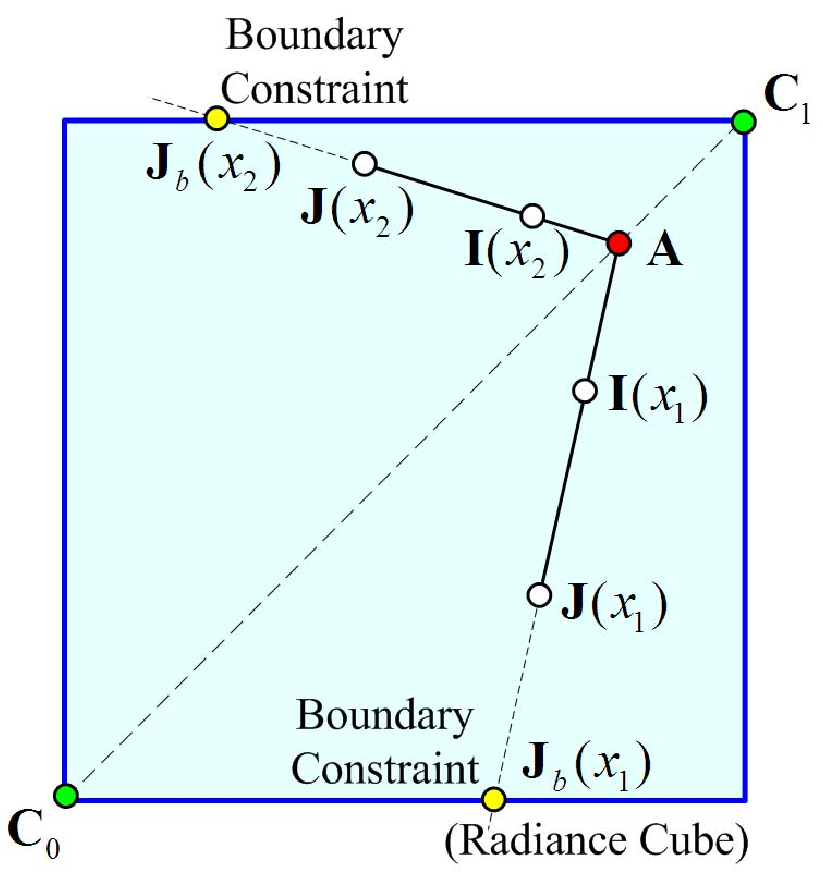
\includegraphics[width=0.8\textwidth]{./imgs/g712.png}
    \caption{约束传递函数(其中$J(x) = I_h^c(x,y)$)}
    \label{fig-trans-c}
 \end{figure}

\begin{equation}
    t_r^* = \text{IFFT-2D}\left(\frac{\frac{\lambda}{\beta}\text{FFT-2D}(\hat t_r) + \sum\limits_{j\in k}\overline{\text{FFT-2D}(D_j)}\text{FFT-2D}(u_j)}{\frac{\lambda}{\beta} + \sum\limits_{j\in k}\overline{\text{FFT-2D}(D_j)}\text{FFT-2D}(u_j)}\right)
    \label{eq-trans-c}
\end{equation}

\begin{equation}
    D_j = \text{circularFilter}(\text{FFT-2D}(t_r), k_j)\quad(j\in k)
    \label{eq-dj}
\end{equation}

\begin{equation}
    u_j = \max{(\lvert D_j\rvert - \frac{W_j}{\text{length}(k)\times\beta} ,0)}\times \text{sign}(D_j)\quad(j\in k)
    \label{eq-uj}
\end{equation}

\begin{equation}
    W_j = e^{\frac{\text{circularFilter}(I_h^c(x,y), filter_j)}{2\sigma^2}}\quad(j\in k)
    \label{eq-wj}
\end{equation}

修正$t_r$如公式\eqref{eq-trans-c}表示其中$\lambda$为正则化系数,$\beta$为权重因子$k$为不同的滤波器核。公式\eqref{eq-dj}\eqref{eq-uj}\eqref{eq-wj}为一些变量的计算式,$\sigma$为预设方差。

根据图\ref{fig-dehazy}的流程,我们可以编写出BCL算法伪代码\ref{algo-BCL}。

\begin{algorithm}[t]
    \caption{BCL}
    \label{algo-BCL}
    \textbf{输入:} 有雾图像$I_h^c(x,y)$,滤波器核大小$W$,大气光上下界$C_1,C_0$,传递函数矫正系数$\epsilon\neq1$
    \begin{algorithmic}
    \State 对有雾图像进行最小值滤波,获取$I_m^c(x,y)$,$I_h^c(x,y)$的最大值就是每个通道的$A_r^c$
    \State 估计传递函数$\hat t_r(x,y) = \max{(\frac{A_r^c - I_h^c(x,y)}{A_r^c - C_0},\frac{I_h^c(x,y)-A_r^c}{C_1 - A_r^c})}$,对传递函数做$3\times 3$的腐蚀
    \State 使用公式\eqref{eq-trans-c}对加约束与规范化获取$t_r(x,y)$,矫正最终传递函数$t_r(x,y) = t_r(x,y)^\epsilon$
    \State 根据大气光$A_r^c$与传递函数$t_r(x,y)$估计去雾图像$\hat I^c(x,y) = \frac{I_h^c(x,y) - A_r^c}{t} + A_r^c$
    \State \Return 去雾图像$\hat I^c(x,y)$
    \end{algorithmic}
\end{algorithm}

\subsection{彩色椭球先验}
彩色椭球先验(Color Ellipsoid Prior,CEP)是一种基于统计的的单图像去雾算法,在218年被Bui等人提出\cite{bui.kim201802}。它一种基于模型的双色去雾方法,该方法在统计上对图像信号随机性具有鲁棒性,在各种雾度范围内有效执行,不需要任何后期细化过程,并且不会产生任何明显可见的噪声或光环工件。他们将 RGB 空间中的像素向量簇拟合到由像素值的矩构造的统计颜色椭圆体,提高了算法稳健性。所提出的方法不是为先验向量选择像素,而是使用椭球几何计算先验向量。计算出的先验向量在椭球表面的向量中具有最小的颜色分量,以便在大多数像素不饱和的任何程度的雾度中最大化去雾像素的对比度。为了避免光晕伪影,他们将模糊过程嵌入到彩色椭圆体的构造中,而不是应用高度复杂的后处理。以上先验向量在线性空间可表示为图\ref{fig-cep}形式。

\begin{figure}[htbp]
    \centering
    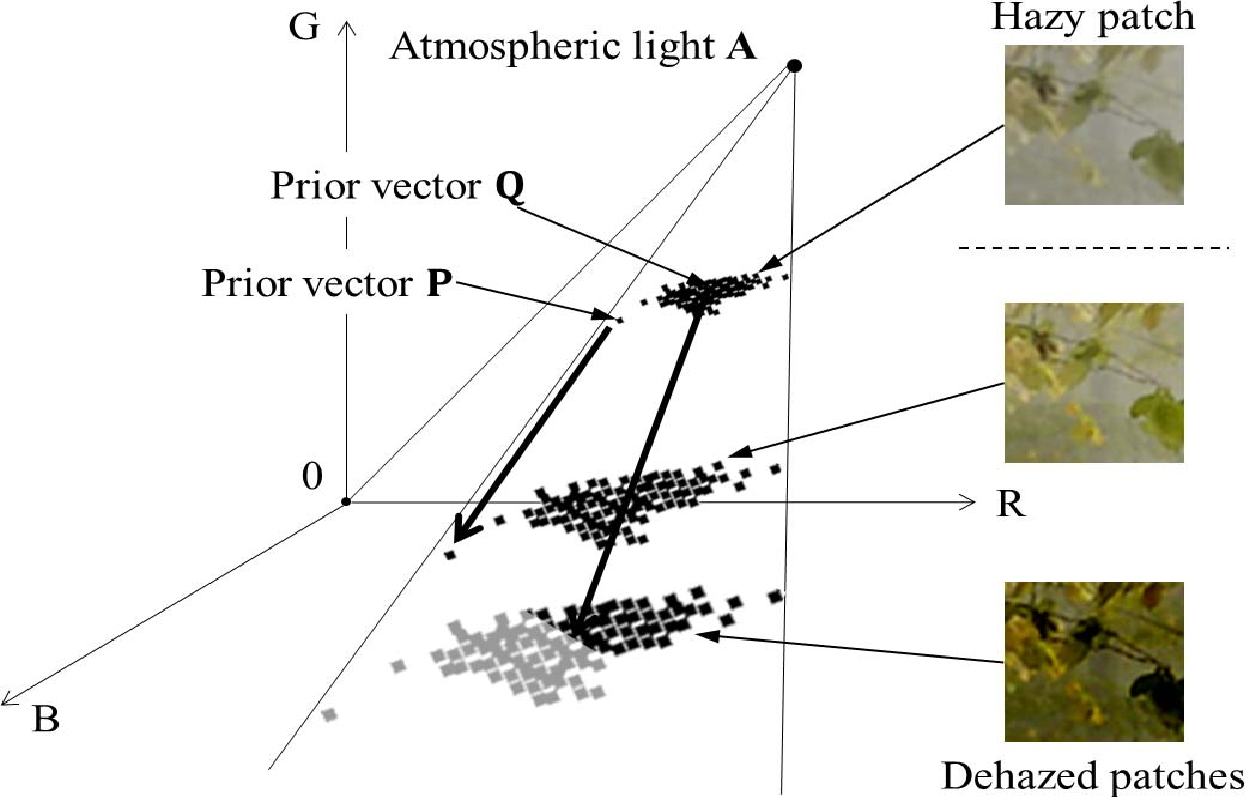
\includegraphics[width=0.8\textwidth]{./imgs/g713.png}
    \caption{椭球几何先验向量}
    \label{fig-cep}
 \end{figure}


 根据图\ref{fig-dehazy}的流程,我们可以编写出CEP算法伪代码\ref{algo-CEP}。

 \begin{algorithm}[t]
     \caption{CEP}
     \label{algo-CEP}
     \textbf{输入:} 有雾图像$I_h^c(x,y)$,滤波器核大小$W$,估计大气光使用的像素比例$p$,透视雾保留系数$\omega$
     \begin{algorithmic}
     \State 对有雾图像进行方框滤波,获取最小$pMN\dim$个像素的位置,根据有雾图像中对应的位置的像素值估计每个通道的$A_r^c$
     \State 使用导向滤波器/方形滤波器(快速)算椭圆向量,估计传递函数$\hat t_r(x,y)$
     \State 修正传递函数$t_r(x,y) = 1 - \omega\times \hat t_r(x,y)$
     \State 根据大气光$A_r^c$与传递函数$t_r(x,y)$估计去雾图像$\hat I^c(x,y) = \frac{I_h^c(x,y) - A_r^c}{t} + A_r^c$
     \State \Return 去雾图像$\hat I^c(x,y)$
     \end{algorithmic}
 \end{algorithm}
\subsection{非线性边界函数的传输下界}
Raikwar等人\cite{raikwar.tapaswi2020}在Meng等人\cite{meng.pan201312}基础上,提出了一种非线性的边界约束方法(记作NLB),通过理论计算出准确的传输函数的下界,进一步优化了算法。他们所提出的方法通过将传输估计问题转化为有雾图像和无雾图像之间的差异估计,来提高准确性。相比于BCL,NLB主要是修改了传输函数的估计(见公式\eqref{eq-tr-low}与\eqref{eq-delta}),次要变化为修改了以下滤波器组的核系数与假定了每个通道的环境光是一致的(见公式\eqref{eq-a})。

\begin{equation}
    \delta = \frac{1}{\min\limits_{c}I_h^c(x,y)} + \epsilon(x,y)
    \label{eq-delta}
\end{equation}

\begin{equation}
    A_r = \max{(A_r^r,A_r^g,A_r^b)}
    \label{eq-a}
\end{equation}

\begin{equation}
    t_r^{low}(x,y) = \frac{1}{1 + \frac{\max{(\min\limits_{c}I_h^c(x,y))}\times 10^{-0.05\zeta\delta}}{A_r - \min\limits_{c}I_h^c(x,y)}}
    \label{eq-tr-low}
\end{equation}

\begin{equation}
    \hat t_r(x,y) = \left\{\begin{matrix}t_r^{low}(x,y), & \text{if } A_r - \min\limits_{c}I_h^c(x,y) > 0.\\
        \frac{\lvert t_r^{low}(x,y) \rvert}{z}, & \text{otherwise}\\\end{matrix}\right. \qquad z = \max \lvert t_r^{low}(x,y) \rvert
    \label{eq-tr-nlb}
\end{equation}

根据图\ref{fig-dehazy}的流程,我们可以编写出NLB算法伪代码\ref{algo-NLB}。

\begin{algorithm}[ht]
    \caption{NLB}
    \label{algo-NLB}
    \textbf{输入:} 有雾图像$I_h^c(x,y)$,滤波器核大小$W$,传递函数矫正系数$\epsilon\neq1$,下界估计参数$\zeta$
    \begin{algorithmic}
    \State 对有雾图像进行最小值滤波,获取$I_m^c(x,y)$,$I_h^c(x,y)$的最大值就是每个通道的$A_r^c$
    \State 根据公式\eqref{eq-tr-low}估计传递函数下界$t_r^{low}(x,y)$,对传递函数做$3\times 3$的腐蚀
    \State 根据公式\eqref{eq-tr-nlb}估计传递函数$\hat t_r(x,y)$,对传递函数做$3\times 3$的腐蚀
    \State 使用公式\eqref{eq-trans-c}对加约束与规范化获取$t_r(x,y)$,矫正最终传递函数$t_r(x,y) = t_r(x,y)^\epsilon$
    \State 根据大气光$A_r^c$与传递函数$t_r(x,y)$估计去雾图像$\hat I^c(x,y) = \frac{I_h^c(x,y) - A_r^c}{t} + A_r^c$
    \State \Return 去雾图像$\hat I^c(x,y)$
    \end{algorithmic}
\end{algorithm}
\section{仿真结果与分析}
\subsection{主观评价}

去雾的图片来自于RESIDE\cite{li2019benchmarking}的HSTS数据集,从图\ref{fig-dehazy}的效果来看,不同的去雾算法都实现了去雾的功能。SID方法都基于强大的假设和先验。这些方法只有在假设为真时才会表现良好。由于这些假设或先验的失败,SID 方法缺乏准确性。通常,通过使用平滑来提高传输的精度,然后降低去雾的计算速度。此外,可以使用先验或通过估计无雾图像的最小颜色通道来估计透射率。先验只有在假设为真时才会表现良好,而最小颜色通道的估计误差会随着雾度密度的增加而增加。这种不准确会导致可见度降低和颜色失真。从图上看前几种算法就出现了可见度降低和颜色失真,即便由于超参设置问题它们在后面的PSNR与SSIM指标中比NLB的方法更高(理论上客观指标也是最高的),主观感受中NLB的方法也是最佳的。

\begin{figure}[htbp]
    \centering
    \subfloat[有雾图]{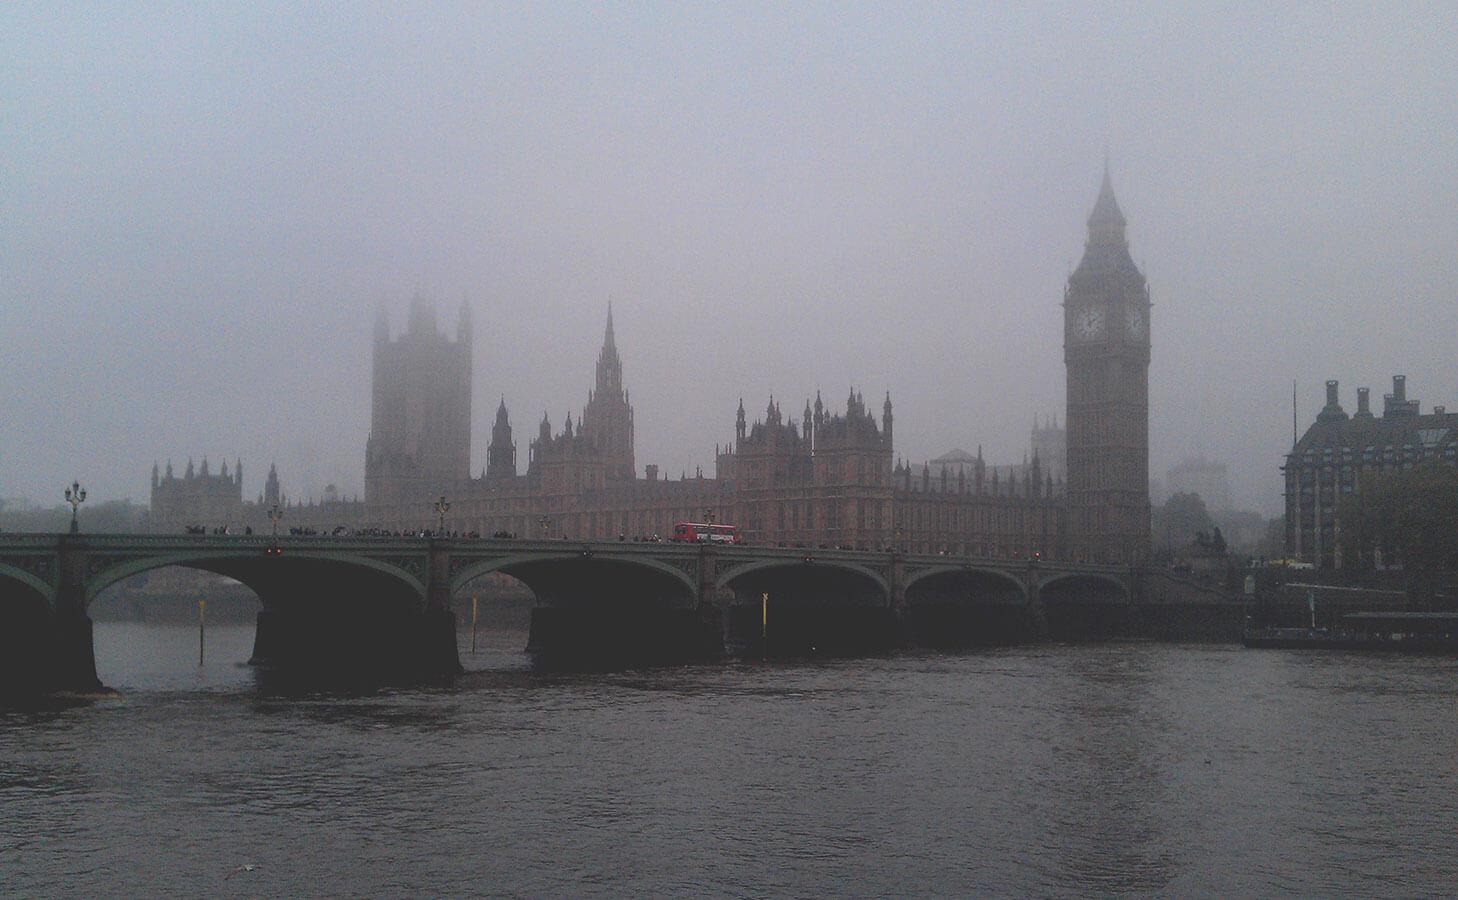
\includegraphics[width=0.3\textwidth]{../data/HSTS_real-world/HazyDr_Google_396.jpeg}}\quad
    \subfloat[DCP
        ]{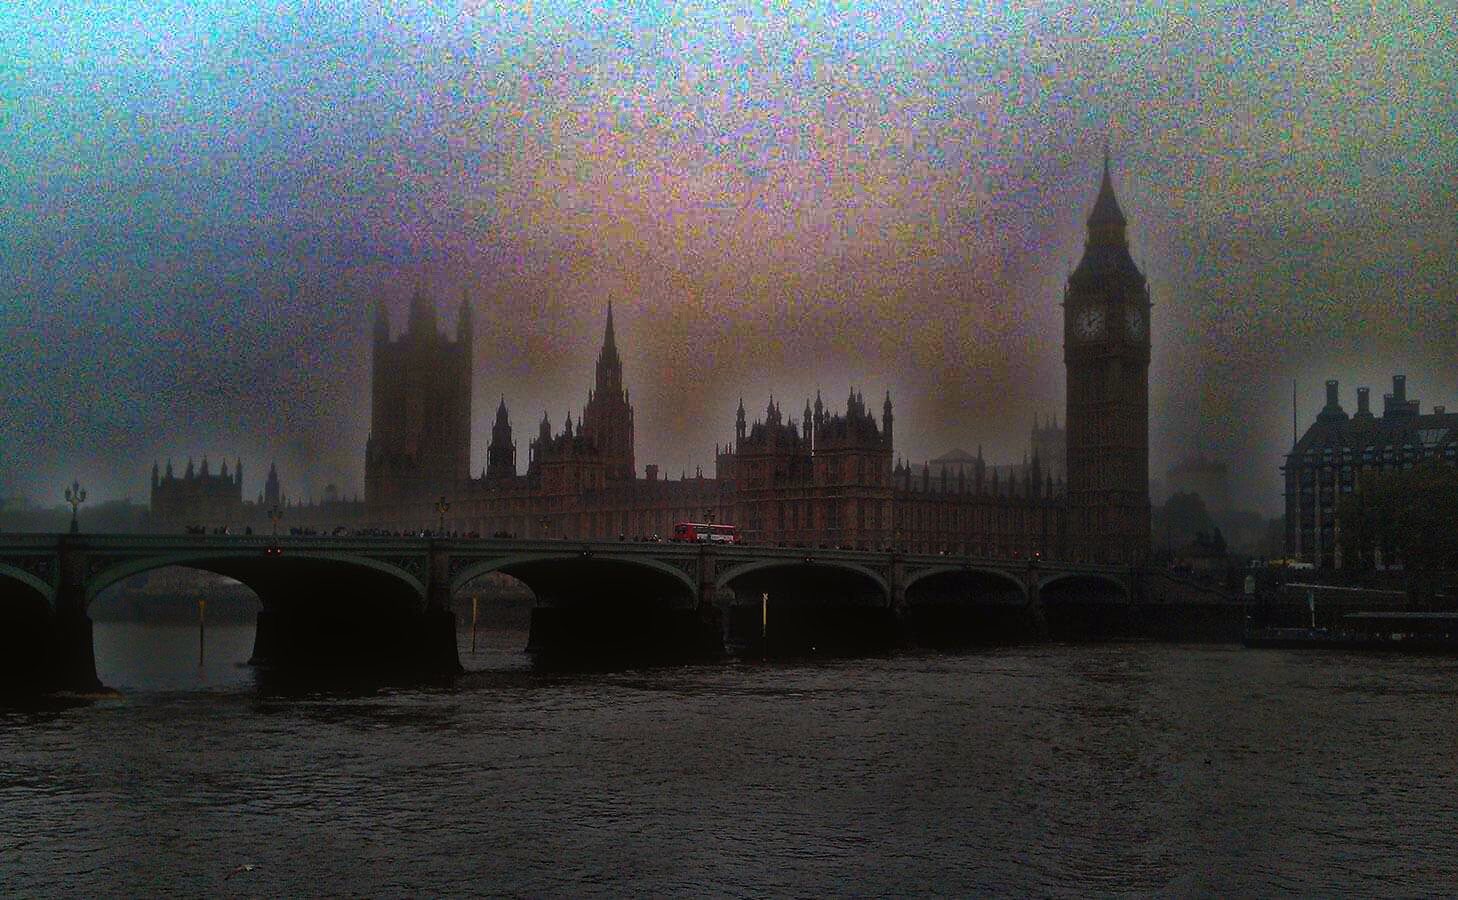
\includegraphics[width=0.3\textwidth]{../output/HSTS_real-world/H_HazyDr_Google_396.jpeg}}
    \quad\subfloat[BCL]{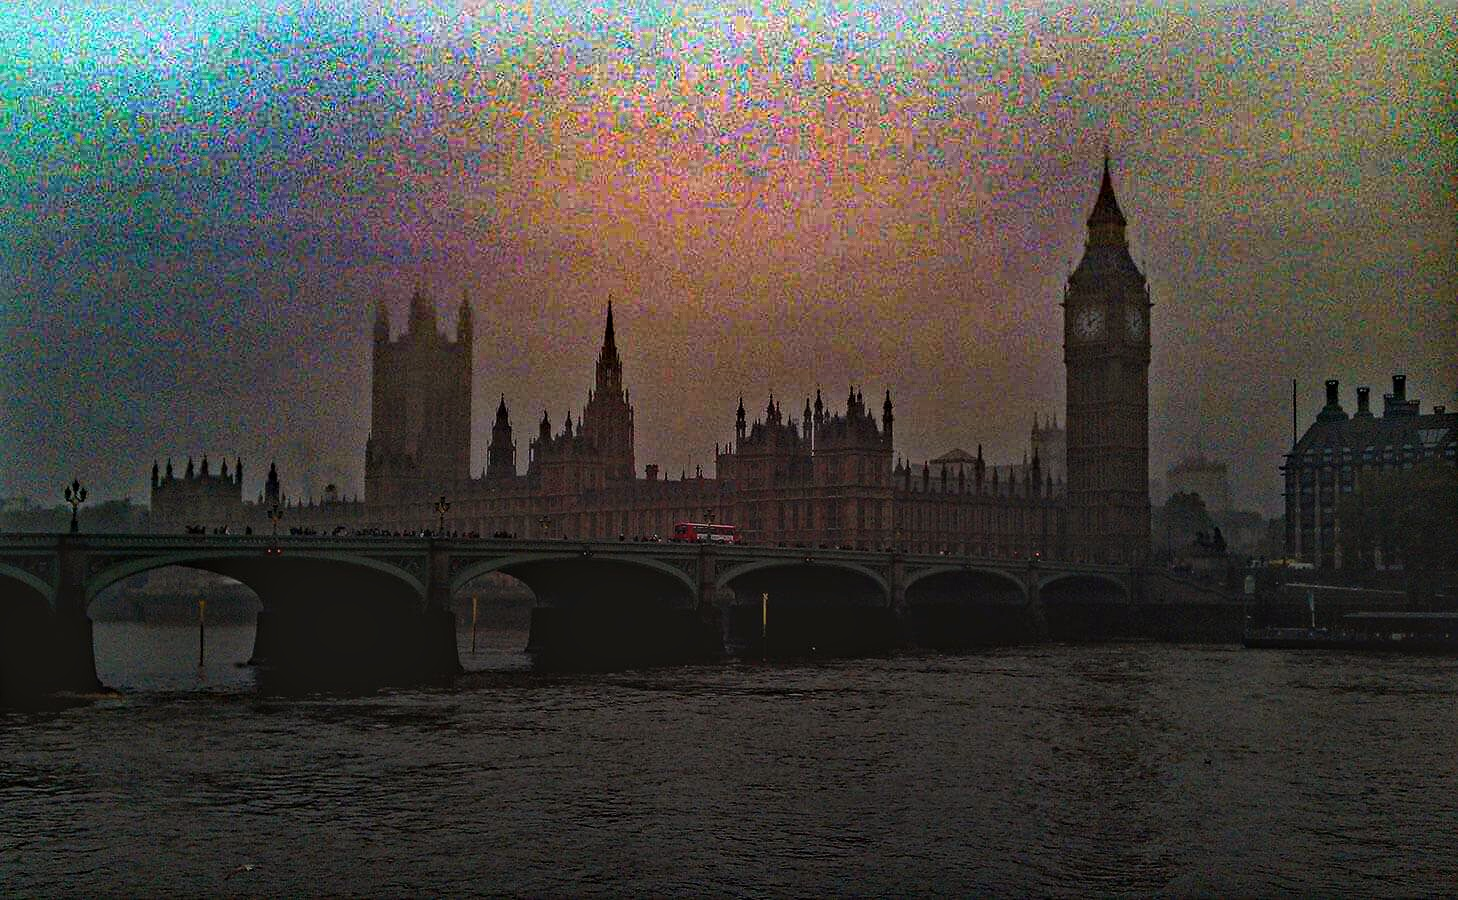
\includegraphics[width=0.3\textwidth]{../output/HSTS_real-world/M_HazyDr_Google_396.jpeg}}
    \\
    \subfloat[CEP]{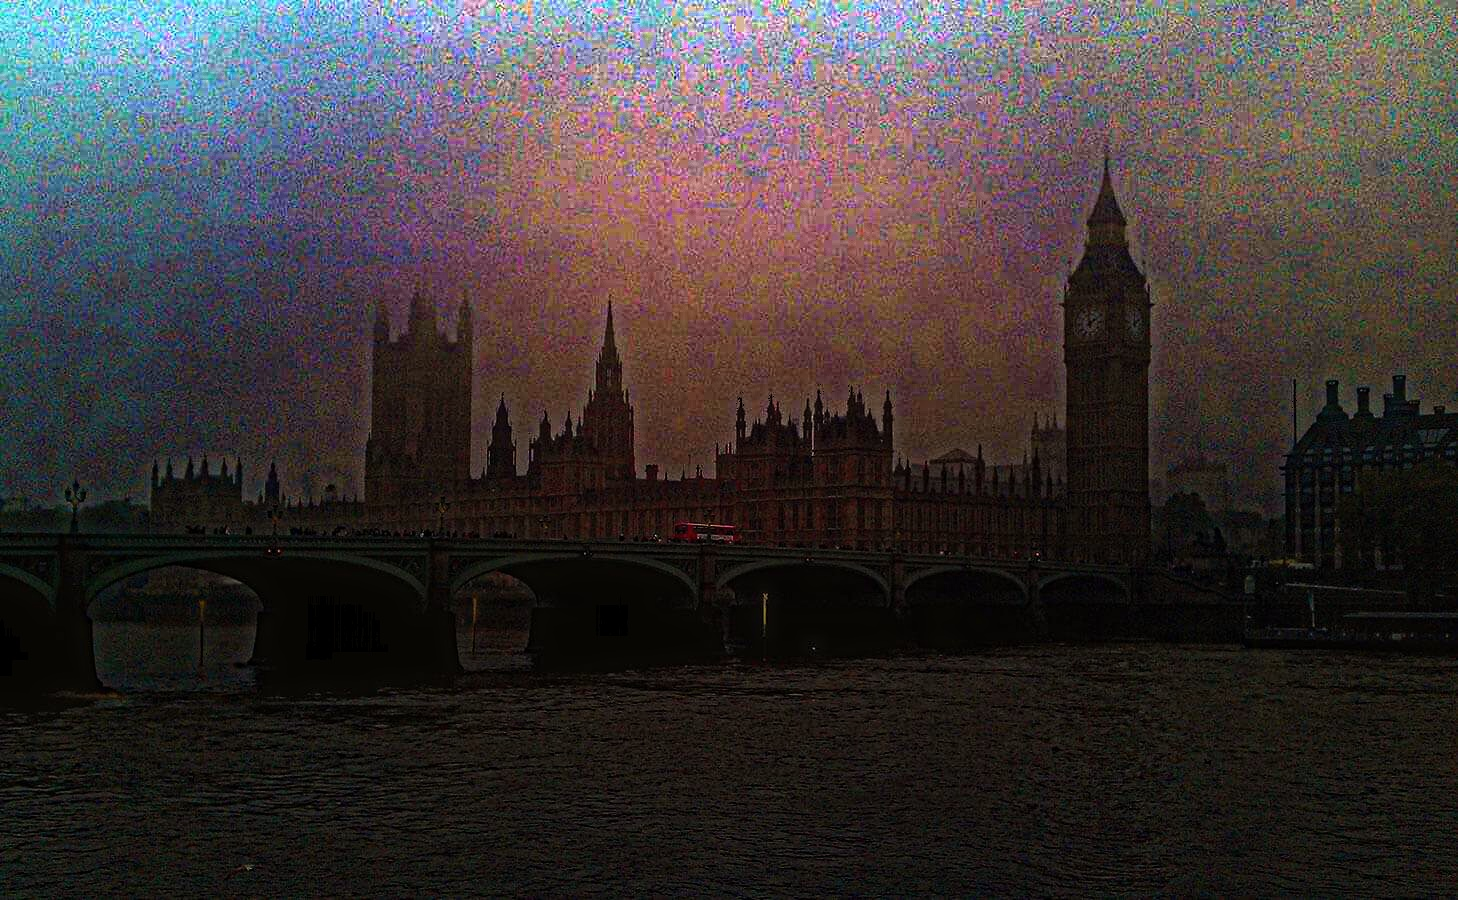
\includegraphics[width=0.3\textwidth]{../output/HSTS_real-world/CEP_HazyDr_Google_396.jpeg}}\quad
    \subfloat[CEP-fast]{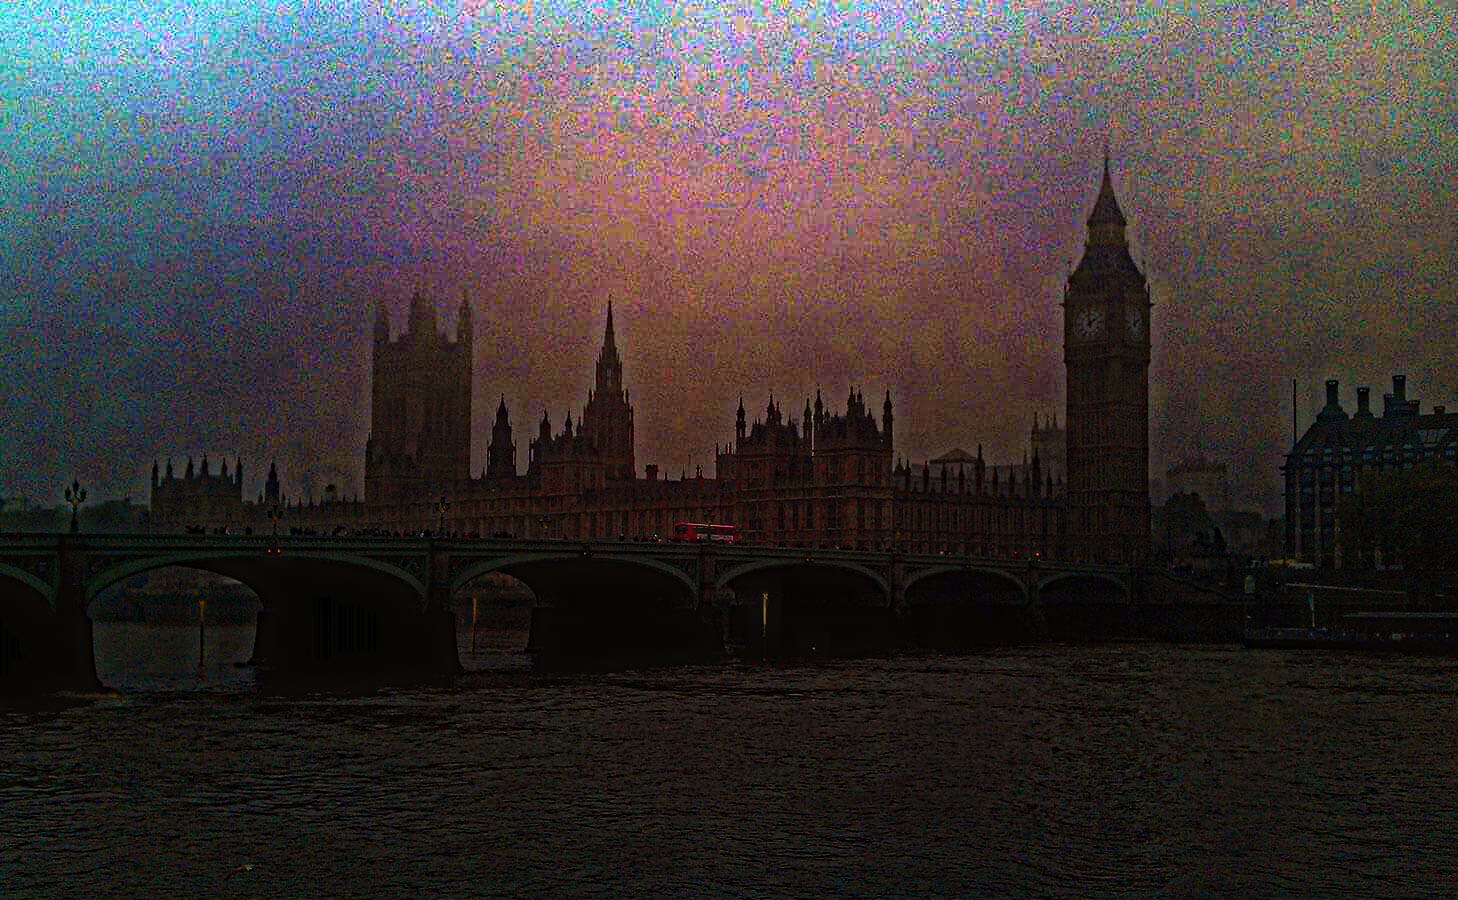
\includegraphics[width=0.3\textwidth]{../output/HSTS_real-world/CEPf_HazyDr_Google_396.jpeg}}
    \quad\subfloat[NLB]{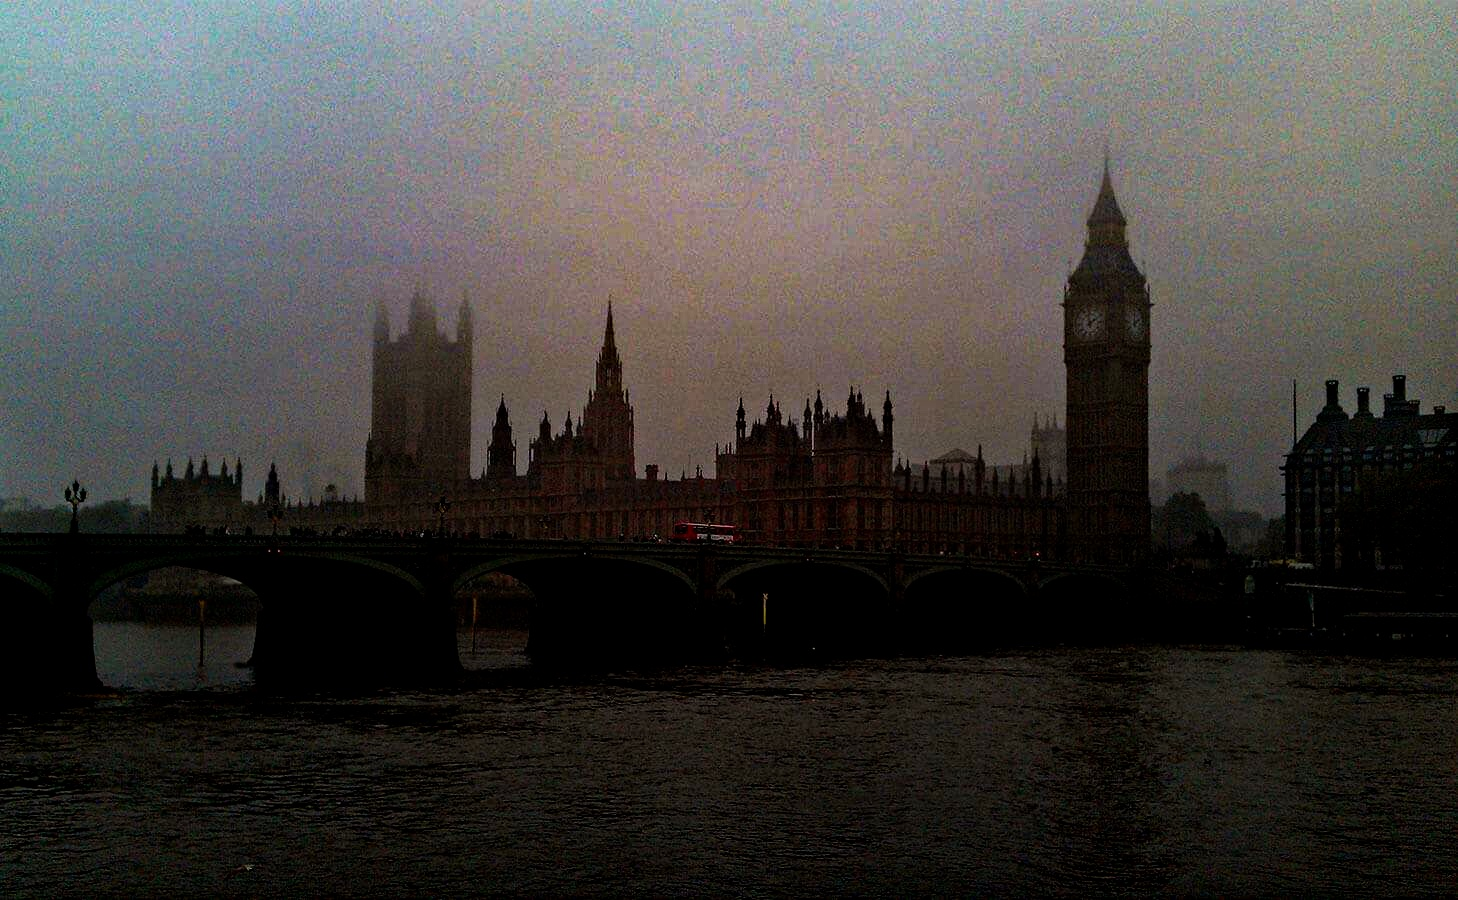
\includegraphics[width=0.3\textwidth]{../output/HSTS_real-world/R_HazyDr_Google_396.jpeg}}
    \\
    \caption{去雾算法结果对比\label{fig-dehazy-cmp}}
\end{figure}

\subsection{客观评价}

\begin{table}
    \caption{SOTS-outdoor数据集下的各算法平均PSNR以及SSIM对比\label{table-cmp}}
    \centering
    \renewcommand{\arraystretch}{2.5} 
    \begin{tabular}{ccc}
        \toprule
        算法 &  PSNR & SSIM \\
        \midrule
        DCP  & $16.9763$ &   $0.8579$  \\
        BCL  & $13.9201$ & $0.7707$\\
        CEP                 & $13.1408$ & $0.6945$\\
        CEP(fast)           & $12.9593$ & $0.6858$\\
        NLB & $14.7957$ & $0.6584$ \\
        \bottomrule
    \end{tabular}
\end{table}

从表\ref{table-cmp}中我们可以获知不同算法在SOTS-outdoor数据集的PSNR与SSIM表现,从表中我们可以获知,复现结果相对合理,与原图由较高的相似性。但是由于没有怎么调整超参数,因此本文复现的效果可能与原文展现的相差甚远,各算法在原文的对比关系可能不太成立,本文复现效果不佳可以归咎于没有像超参,我曾调整过NLB在去雾步骤的$\delta$参数,两个指标都能提升一大截,由于时间不足,没空精调了,为本课程的大作业留下一个遗憾。


\section{总结}
\label{s5}
在本次期末大作业,本人复现了以上的几种算法,其中NLB算法\cite{raikwar.tapaswi2020}我无法复现出作者声称的计算速度,即便是他们给予的源码也远远达不到声称的计算速度,对该算法的计算速度方面保持一定的怀疑态度。经过本次本次的作业,对图像去雾等领域有了更深的了解,本文的工作可总结为以下两点:
\begin{itemize}
    \item 了解了图像去雾的需求与从大气散射模型的角度了解了雾与霾对图像的影响。

    \item 了解了几种SID算法,并复现了它们,并以合适的度量进行了对比。
\end{itemize}

但是由于时间关系以及复现的算法较多,我只是粗略地复现了它们,没有实现论文中展示的指标,没有实现100\%的完成度,留下一点遗憾与不足。
\endgroup

\medskip
{\small{}\bibliographystyle{unsrt}
\bibliography{report}
}{\small\par}

%%%%%%%%%%%%%%%%%%%%%%%%%%%%%%%%%%%%%%%%%%%%%%%%%%%%%%%%%%%%



% \appendix


% \section{Appendix}
% \textit{proof} Theorem~\ref{thm31}

\end{document}